\vspace{10pt}
\subsection*{\bi KAGRA Project Status}
\vspace{3pt}
\noindent {\sf [Spokesperson :\ Takashi UCHIYAMA]}

\vspace{3pt}
\noindent {\sf \small ICRR, The Univ.\ of Tokyo, Hida, Gifu 506-1205}

\subsubsection*{\bf Overview}
KAGRA, Large-scale Cryogenic Gravitational wave Telescope, aims at detecting gravitational waves and developing gravitational wave astronomy, which was established by the first detection of gravitational waves by LIGO. KAGRA employs a 3\,km L-shaped laser interferometer with a cryogenic mirror system placed underground at Kamioka\cite{kagra_review}. The KAGRA development is divided into two stages: the initial KAGRA (iKAGRA) and baseline KAGRA (bKAGRA). The iKAGRA interferometer is a simple Michelson interferometer with a 2-Watt laser, room-temperature mirrors, and a simple vibration isolation system. We completed the iKAGRA interferometer with a test run in April 2016\cite{ikagra_paper}. Then we proceeded to bKAGRA. 






Figure~\ref{fig:config} and \ref{fig:vis} show a schematic view of optical layout of the bKAGRA interferometer and the KAGRA vibration isolation systems. Table \ref{table:design_para} shows design parameter of the bKAGRA interferometer\cite{phase1_paper}. The bKAGRA interferometer will employ a Resonant Sideband Extraction (RSE) interferometer with 180-Watt laser, cryogenic Sapphire mirrors, and several kinds of vibration isolation systems. The bKAGRA interferometer should attain the sensitivity high enough for the detection of gravitational waves with the help of the high power laser and RSE interferometer to reduce the quantum noise, the cryogenic Sapphire mirrors to reduce the thermal noise, and the vibration isolation systems to reduce the seismic noise. Figure~\ref{fig:kagra-sensitivity} shows designed sensitivities of bKAGRA in case of Broadband RSE (BRSE) and of Detuned RSE (DRSE), where incoherent sum of the fundamental noise sources is assumed. Observation range for an in-spiral and merger of neutron-star binary reaches 135\,Mpc in BRSE and 153\,Mpc in DRSE with the same definition of the observation range as LIGO and Virgo. 


\begin{figure}
\begin{center}
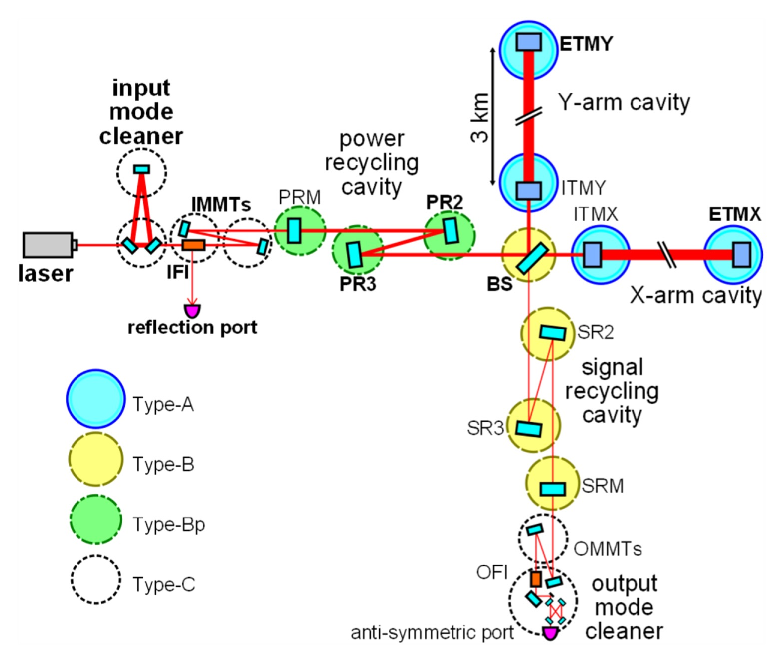
\includegraphics[width=8.5cm]{astrodiv/gw/overview/fig/kagra_config.eps}
\caption{Schematic view of the bKAGRA interferometer\cite{phase1_paper}. Type-A, Type-B, Type-Bp, and Type-C are the names of vibration isolation system for each mirror. }
\label{fig:config}
\end{center}
\end{figure}




\begin{figure}
\begin{center}
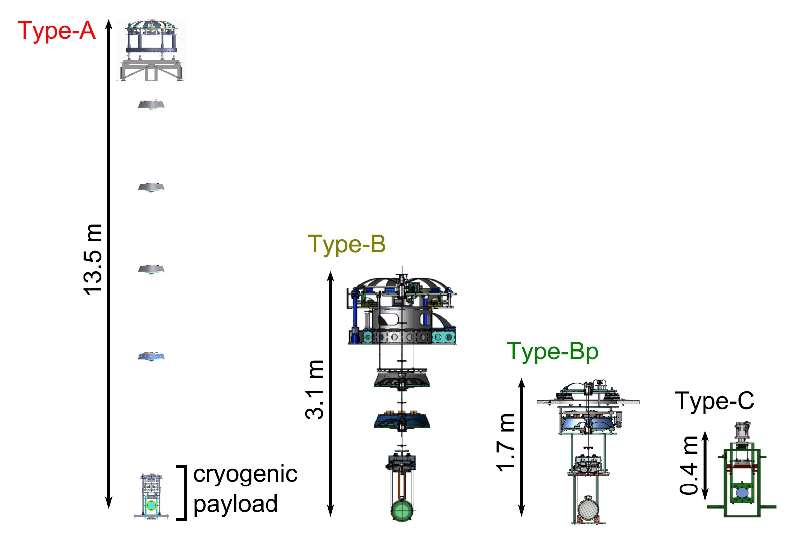
\includegraphics[width=8.5cm]{astrodiv/gw/overview/fig/suspensions.eps}
\caption{KAGRA vibration isolation systems\cite{phase1_paper}. KAGRA equips four kinds of vibration isolation systems such as Type-A, Type-B, Type-Bp, and Type-C.}
\label{fig:vis}
\end{center}
\end{figure}

\begin{table*} 
\begin{center} 
 \caption{\label{table:design_para}The design parameters of the bKAGRA interferometer\cite{phase1_paper}.}
 \begin{tabular}{llll}
  \hline
 Arm cavity length & 3000\,m & Test mass size & $\phi 22\,\mathrm{cm} \times 15\,\mathrm{cm}$ \\
Laser wave length & 1064\,nm & Mass of test mass & 22.8\,kg \\
Input power at PRM & 67W & Temperature of test mass & 22\,K \\
Arm intra-cavity power & 340\,kW & Beam radius at test mass & 3.5\,cm\\ 
ITM transmittance & 0.4\,\% & PRC/SRC lengths & 66.6\,m\\ 
PRM transmittance & 10\,\% & Detuning angle & 3.5\,deg\\  
SRM transmittance & 15\,\% & Homodyne angle & 135.1\,deg\\  \hline
%\hline\hline
\end{tabular}
\end{center} 
 \end{table*}






\begin{figure}
\begin{center}
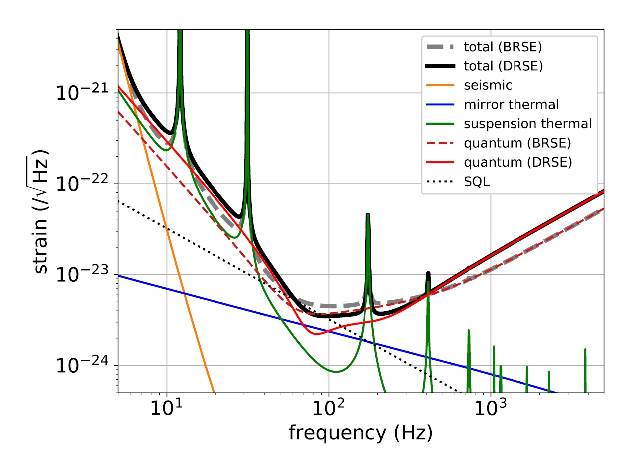
\includegraphics[width=8.5cm]{astrodiv/gw/overview/fig/kagra_sensitivity.eps}
\caption{The designed sensitivity of the bKAGRA interferometer\cite{phase1_paper}. "total", "seismic", "mirror thermal", "suspension thermal", "quantum", and "SQL" mean total sum of fundamental noise sources shown in this figure, seismic noise including gravity gradient noise, mirror thermal noise, suspension thermal noise, quantum noise, and standard quantum limit, respectively. The figure shows "total" and "quantum noise" in both Broadband RSE (BRSE) and Detuned RSE (DRSE) case. Observation range for an in-spiral and merger of neutron-star binary reaches 135\,Mpc in BRSE and 153\,Mpc in DRSE with the same definition of the observation range as LIGO and Virgo.}
\label{fig:kagra-sensitivity}
\end{center}
\end{figure}


Figure~\ref{fig:scenario} shows the international collaborative observation scenario\cite{scenario_paper}. LIGO conducted Observation 1 (O1) from September 12, 2015 to January 19, 2016 and Observation 2 (O2) from November 30, 2016 to August 25, 2017. Virgo joined O2 from August 1, 2017. LIGO and Virgo started Observation 3 (O3) from April 1, 2019. Initially O3 was planned to continue until the end of April in 2020, but it was suspended on March 27, 2020 due to the influence of the COVID-19\cite{o3_suspend}. 

The KAGRA observatory signed the three documents between LIGO and VIRGO in order to realize international joint observation on October 4, 2019. The documents are the Memorandum of Agreement between VIRGO, KAGRA, and LIGO (main part)\cite{moa}, Memorandum of Agreement between VIRGO, KAGRA, and LIGO (Attachment A)\cite{moa_at}, and Letter of Intent for KAGRA to Join the O3 Run\cite{loi_o3}. On the same day, the KAGRA observatory held a completion ceremony.



\begin{figure}
\begin{center}
\includegraphics[width=8.5cm]{astrodiv/gw/overview/fig/scenario.eps}
\caption{International observation scenario\cite{scenario_paper}. LIGO and Virgo  started Observation 3 from April 1 in 2019. }
\label{fig:scenario}
\end{center}
\end{figure}


In FY2019 we started interferometer commissioning works to reach sensitivity required to join O3. The required sensitivity of 1\,Mpc was defined as an observation range of neutron star binary coalescences\cite{loi_o3}. KAGRA reached the required sensitivity almost the end of March 2020. Details of the commissioning works can be found in the "Commissioning" section. Along with the commissioning works the KAGRA observatory carried out several engineering runs and two Observation runs by the end of April 2020. The first observation run was carried out only by KAGRA with the observation range of 0.5\,Mpc from February 25 to March 7, 2020. The second observation run was carried out with GEO600 from April 7 to 21, 2020. This observation called O3GK is regarded as an official joint observation with GEO600 by LIGO, VIRGO, and KAGRA. KAGRA was operated in O3GK with the observation range of almost 0.6\,Mpc and duty factor of 53\,\% has achieved. Details of observation runs can be found in the section of "Observation".



%In FY2018 we started with an operation of KAGRA interferometer as bKAGRA phase 1 which is 3\,km Michelson interferometer with two sapphire mirrors suspended by the Type-A vibration isolation systems. One sapphire mirror was cooled at 18\,K. The operation was done from April 28 to May 6 in 2018 and it was the first demonstration of operating km-class interferometer at cryogenic temperature. Figure~\ref{fig:dutyfactor} and Figure~\ref{fig:phase1_sens} shows a summary of daily status of the operation and a strain sensitivity comparing with noise sources\cite{phase1_paper}, respectively. Duty factor in the first half of the operation reached 88.6\%. The observation range for an in-spiral and merger of neutron-star binary and BH binary reached 17\,pc and 100\,pc, respectively. The longest continuous operation time was 11.1\,hour. 
%
%
%
%
%
%\begin{figure}
%\begin{center}
%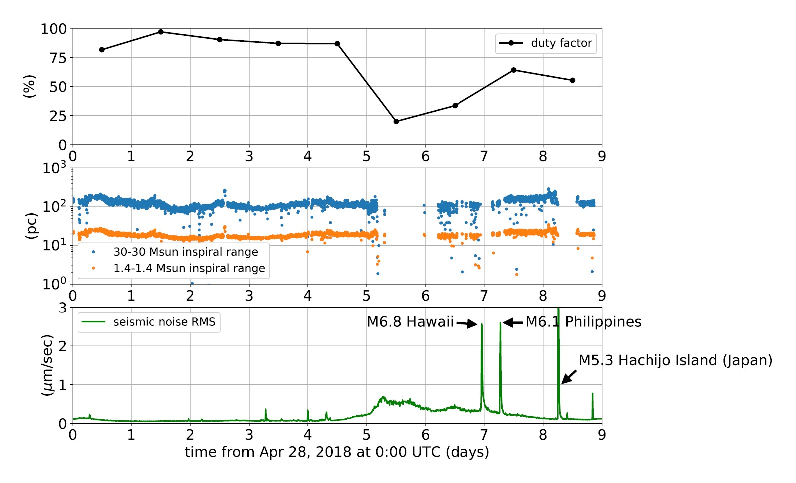
\includegraphics[width=8.5cm]{astrodiv/gw/overview/fig/dutyfactor.eps}
%\caption{Daily status of bKAGRA phase 1 operation\cite{phase1_paper}. The figure shows daily duty factor (Top panel), inspiral range (Middle panel), and seismic noise level (Bottom panel) during the operation. The operation was done from April 28 to May 6 in 2018.}
%\label{fig:dutyfactor}
%\end{center}
%\end{figure}
%
%
%
%
%
%\begin{figure}
%\begin{center}
%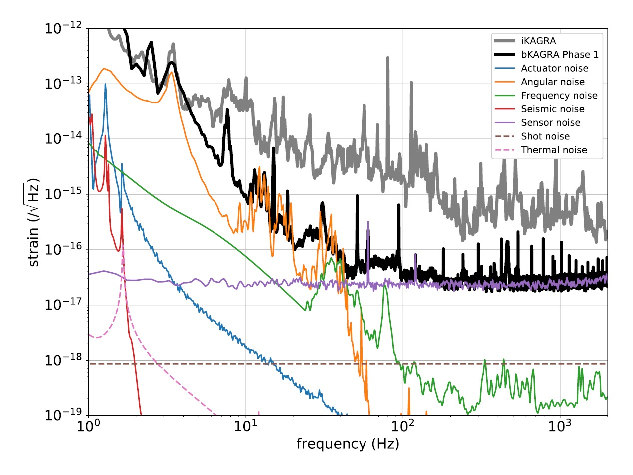
\includegraphics[width=8.5cm]{astrodiv/gw/overview/fig/phase1_sens.eps}
%\caption{Strain sensitivity of KAGRA in phase 1 operation\cite{phase1_paper}. }
%\label{fig:phase1_sens}
%\end{center}
%\end{figure}
%
%
%
%After the bKAGRA phase 1 operation, we started construction of the bKAGRA interferometer with 40\,W laser power. What we have installed were an infrared laser system with the maximum power of 40\,W, two sets of arm length stabilization system using a green laser, calibration systems using photon radiation pressure, large beam baffles, transmission monitor systems, some optics consisting a signal recycling cavity and output optics, two input test masses called ITMX and ITMY in Figure~\ref{fig:config}, and so on. Physical Environmental Monitor (PEM) is a sensor network consisting several kinds of environmental sensors such as accelerometers, seismometers, magnetometers, thermometers, acoustic sound monitors, power monitors and so on. Purpose of PEM is to check the detector health, noise sources, and data quality in cooperation with the detector characterization group. We placed many sensors in the KAGRA site and monitoring has already started. 
%
%
%We have tried lock acquisition of the X-arm cavity for the first time in parallel with the installation works mentioned above. The lock acquisition of the X-arm cavity was successfully achieved with helps of the arm length stabilization system. Then we carried out charcterization of the X-arm cavity. Table\ref{table:xarm} shows a summary of optical parameters of the X-arm cavity comparing with designed and measured values. 
%
%\begin{table*} 
%\begin{center} 
% \caption{\label{table:xarm}Optical parameters of the X-arm cavity\cite{xarm_com}.}
% \begin{tabular}{lll}
% Parameter name & Designed & Measured \\ \hline
% Cavity length & 3000\,m & 29999.990(2)\,m \\
% Finesse for 1064\,nm & 1530 & 1410(30) \\
%Roundtrip loss for 1064\,nm & <100\,ppm & 86(3)\,ppm \\
%Finesse for 532\,nm & 49.2 & 41.0(3) \\ \hline 
%\end{tabular}
%\end{center} 
% \end{table*}

%There are progress reports in this annual report from Vacuum subgroup, Input Output Optics subgroup, Cryogenic subgroup, Digital control System subgroup, Analogue Electronics subgroup, Detector Characterization subgroup, ????, and Data analysis subgroup. 





%& Objects &Unit & Room temperature & Cryogenic  \\ \hline
%& Mirror temperature & K & $299$ & $17\, \textrm{and}\, 18$ \\  \hline
%$W _{\mathrm{front}}$ &Beam spot radius on front mirrors & mm & $4.9$ & $4.9$\\
%$W _{\mathrm{end}}$ &Beam spot radius on end mirrors & mm & $8.5$ & $8.5$\\ \hline
%& Material properties of Sapphire & & & \\ 
%$\alpha$ &Thermal expansion coefficient \cite{data_book, th_expansion_cryo} & 1/K& $5.4 \times 10^{-6}$ & $5.6 \times 10^{-9}$\\
%$\rho C$ &Specific heat per unit volume \cite{data_book} & J/K/m$^{3}$& $3.1 \times 10^{6}$ & $2.8 \times 10^{3}$\\
%$\kappa$ &Thermal conductivity \cite{data_book} & W/m/K& $46$ & $1.6 \times 10^{4}$\\
%$\sigma$ &Poisson's ratio\footnote{We found various values for the Poisson's ratio of sapphire between 0.23 and 0.30. We used the averaged value. 
%}& & $0.27$ & $0.27$\\
%$E$ &Young's modulus \cite{coating_Q}& Pa& $40 \times 10^{10}$ & $40\times 10^{10}$\\ 
%$\phi _{\mathrm{substr}}$ &Mechanical loss \cite{sapphire_subQ}& &  $1/4.6 \times 10^{6}$ & $1/1.5 \times 10^{8}$\\ \hline
%$\phi _{\mathrm{coat}}$ &Mechanical loss in coating films \cite{coating_Q} & & $4.0 \times 10^{-4}$ & $4.0 \times 10^{-4}$\\
%$d$ &Thickness of coating films & $\mathrm{\mu}$ m & $3.9$ & $3.9$\\
%



%In FY2017 we continued several installation and upgrade works toward the bKAGRA Phase 1. Fig. \ref{fig:bkagraphase1} and \ref{fig:vis} shows optical layout of bKAGRA Phase 1 and vibration isolation systems, respectively. We have installed mirrors of PRM, PR2, BS, ETMX, and ETMY in FY2017. ETMX is the sapphire mirror. ETMY is a spare sapphire mirror. PRM, PR2, and BS are made of fused silica. PRM, PR2 have been suspended Type-Bp vibration isolation systems. We have also upgraded the vibration isolation system for PR3 from Type-Bp' to Type-Bp. BS has been suspended by a Type-B vibration isolation system. ETMX and ETMY have been suspended Type-A vibration isolation systems. ETMY has been cooled 18\,K. All the optics needed for bKAGRA Phase 1 have been installed in FY2017 and we have successfully operated the cryogenic 3\,km Michelson interferometer from 28 April of 2018. 





%Here shows some photos about vibration isolation systems and mirrors installed in FY2017.





%\begin{figure}
%\begin{center}
%\includegraphics[width=8.5cm]{astrodiv/gw/overview/fig/bs.eps}
%\caption{Type-B vibration isolation system for beam splitter.}
%\label{fig:bs}
%\end{center}
%\end{figure}
%
%\begin{figure}
%\begin{center}
%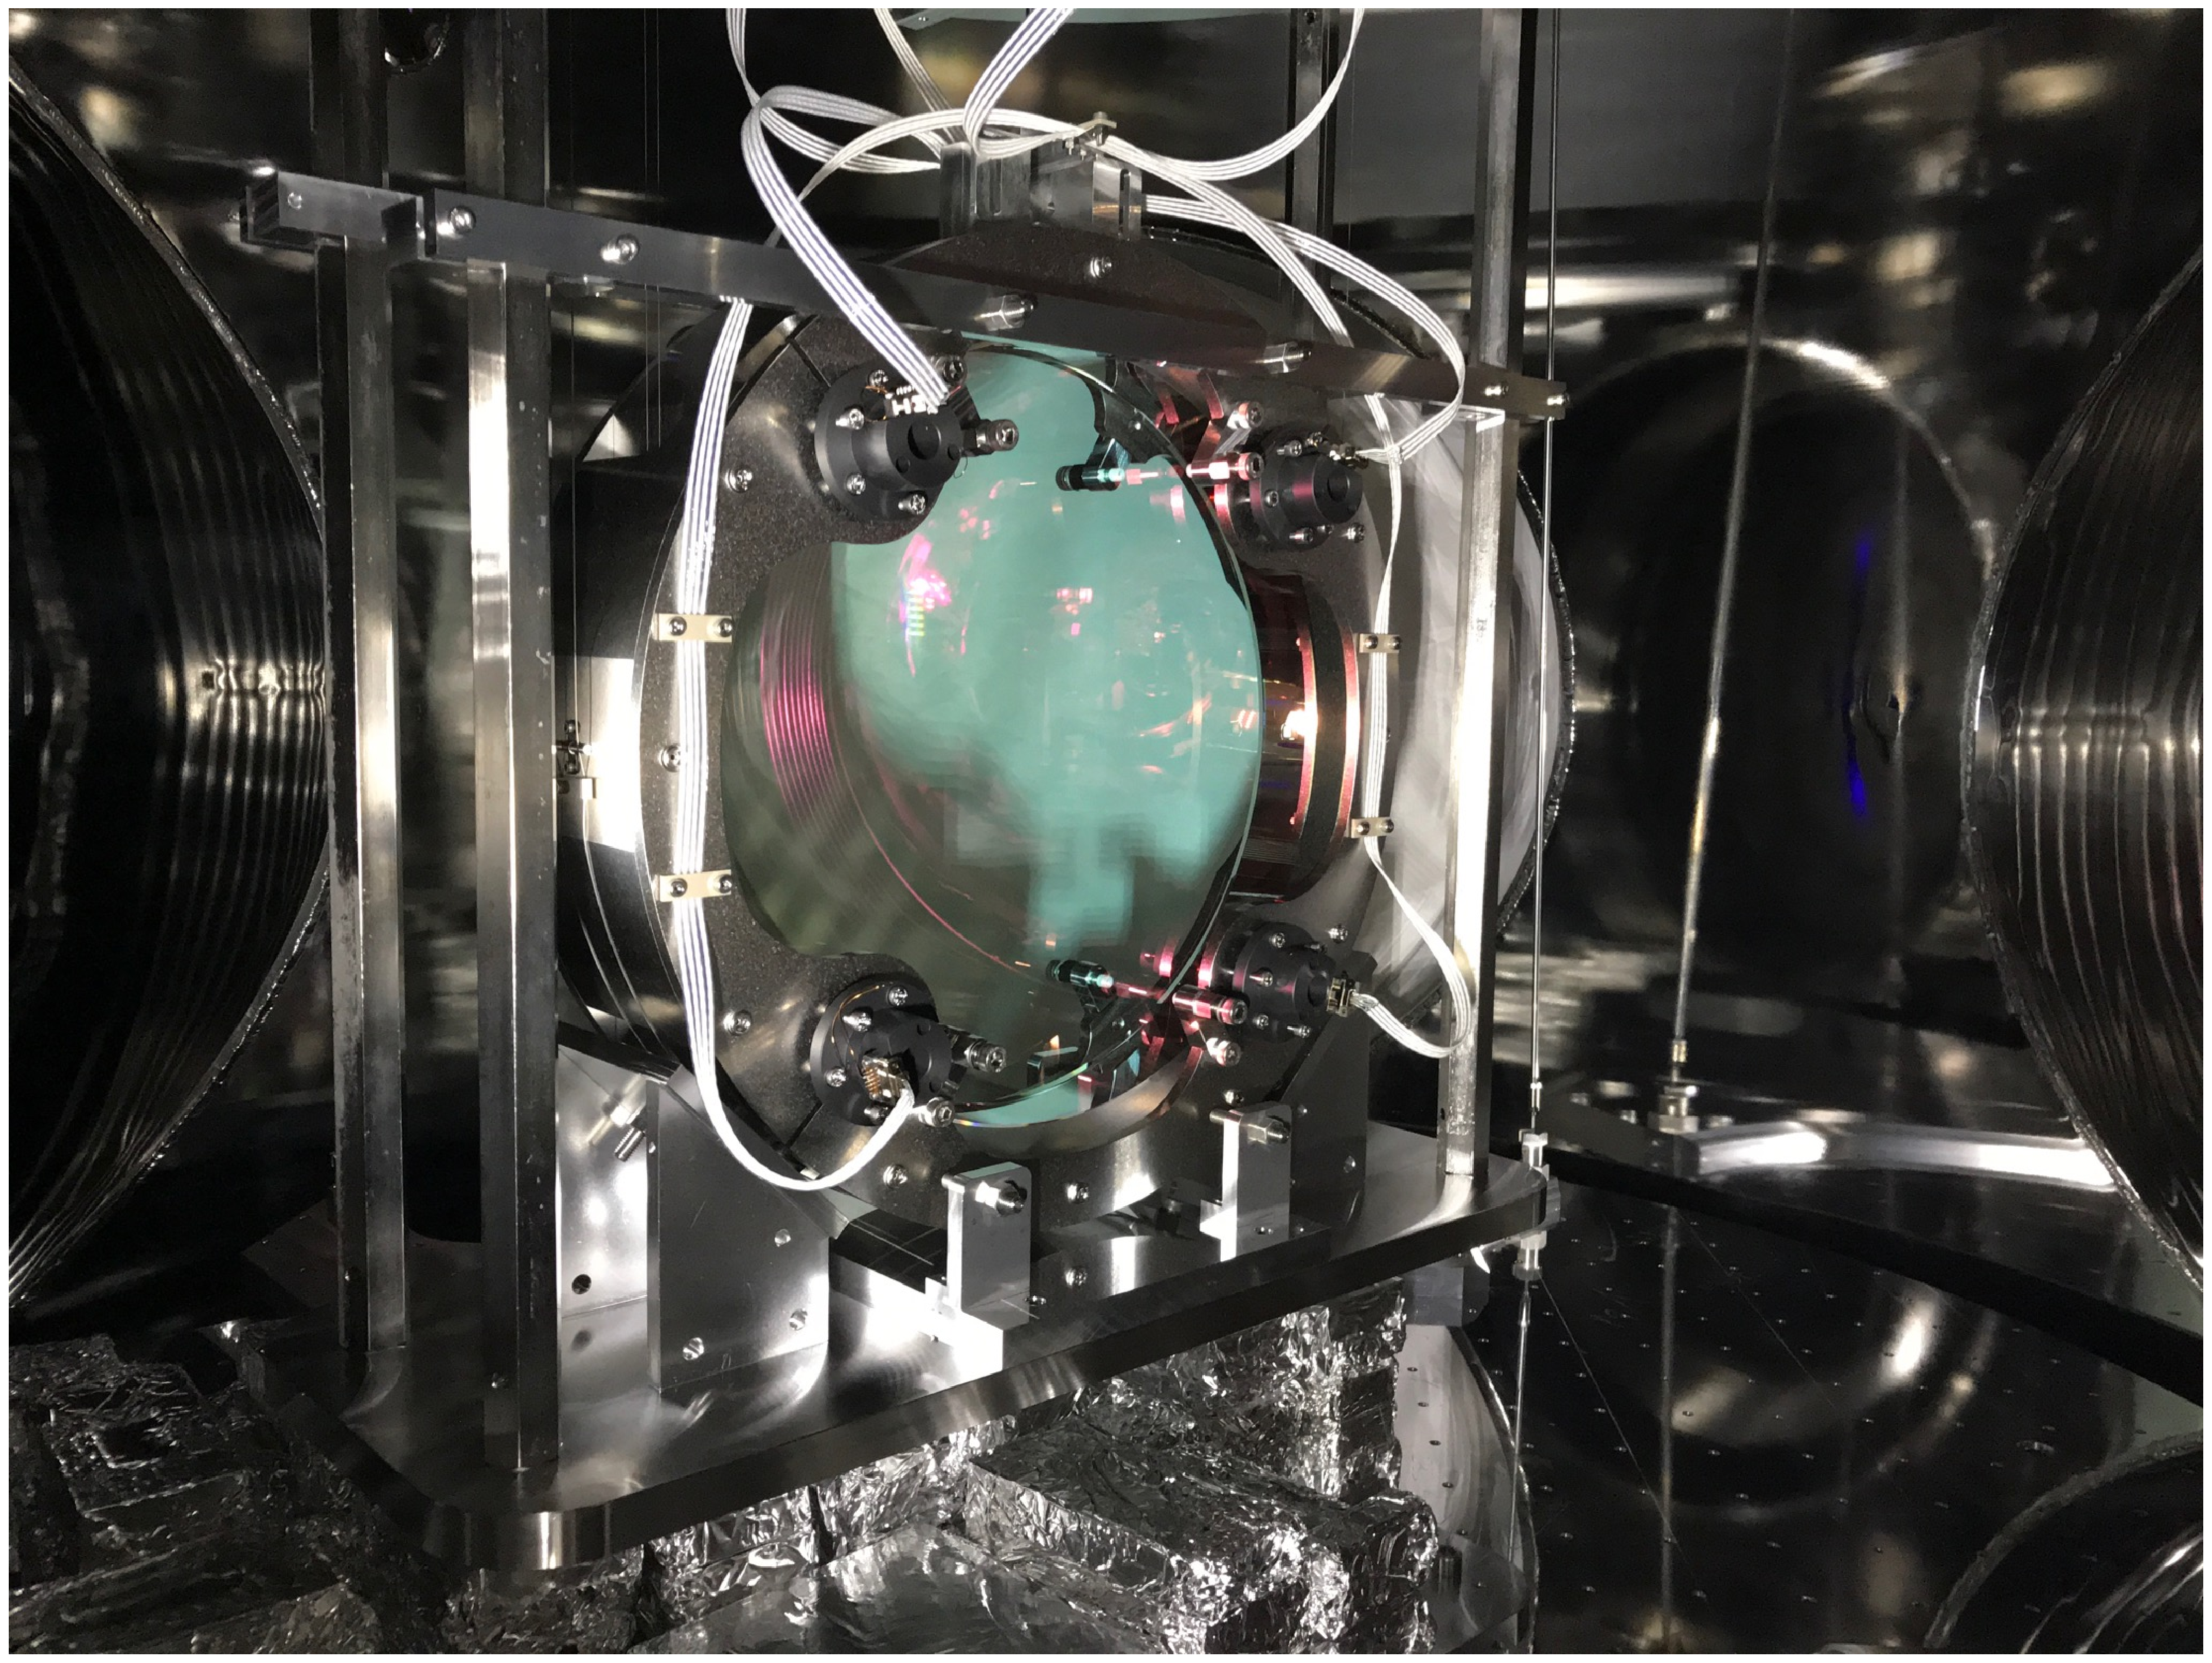
\includegraphics[width=8.5cm]{astrodiv/gw/overview/fig/bs2.eps}
%\caption{Beam splitter suspended in a vacuum chamber.}
%\label{fig:bs}
%\end{center}
%\end{figure}
%
%\begin{figure}
%\begin{center}
%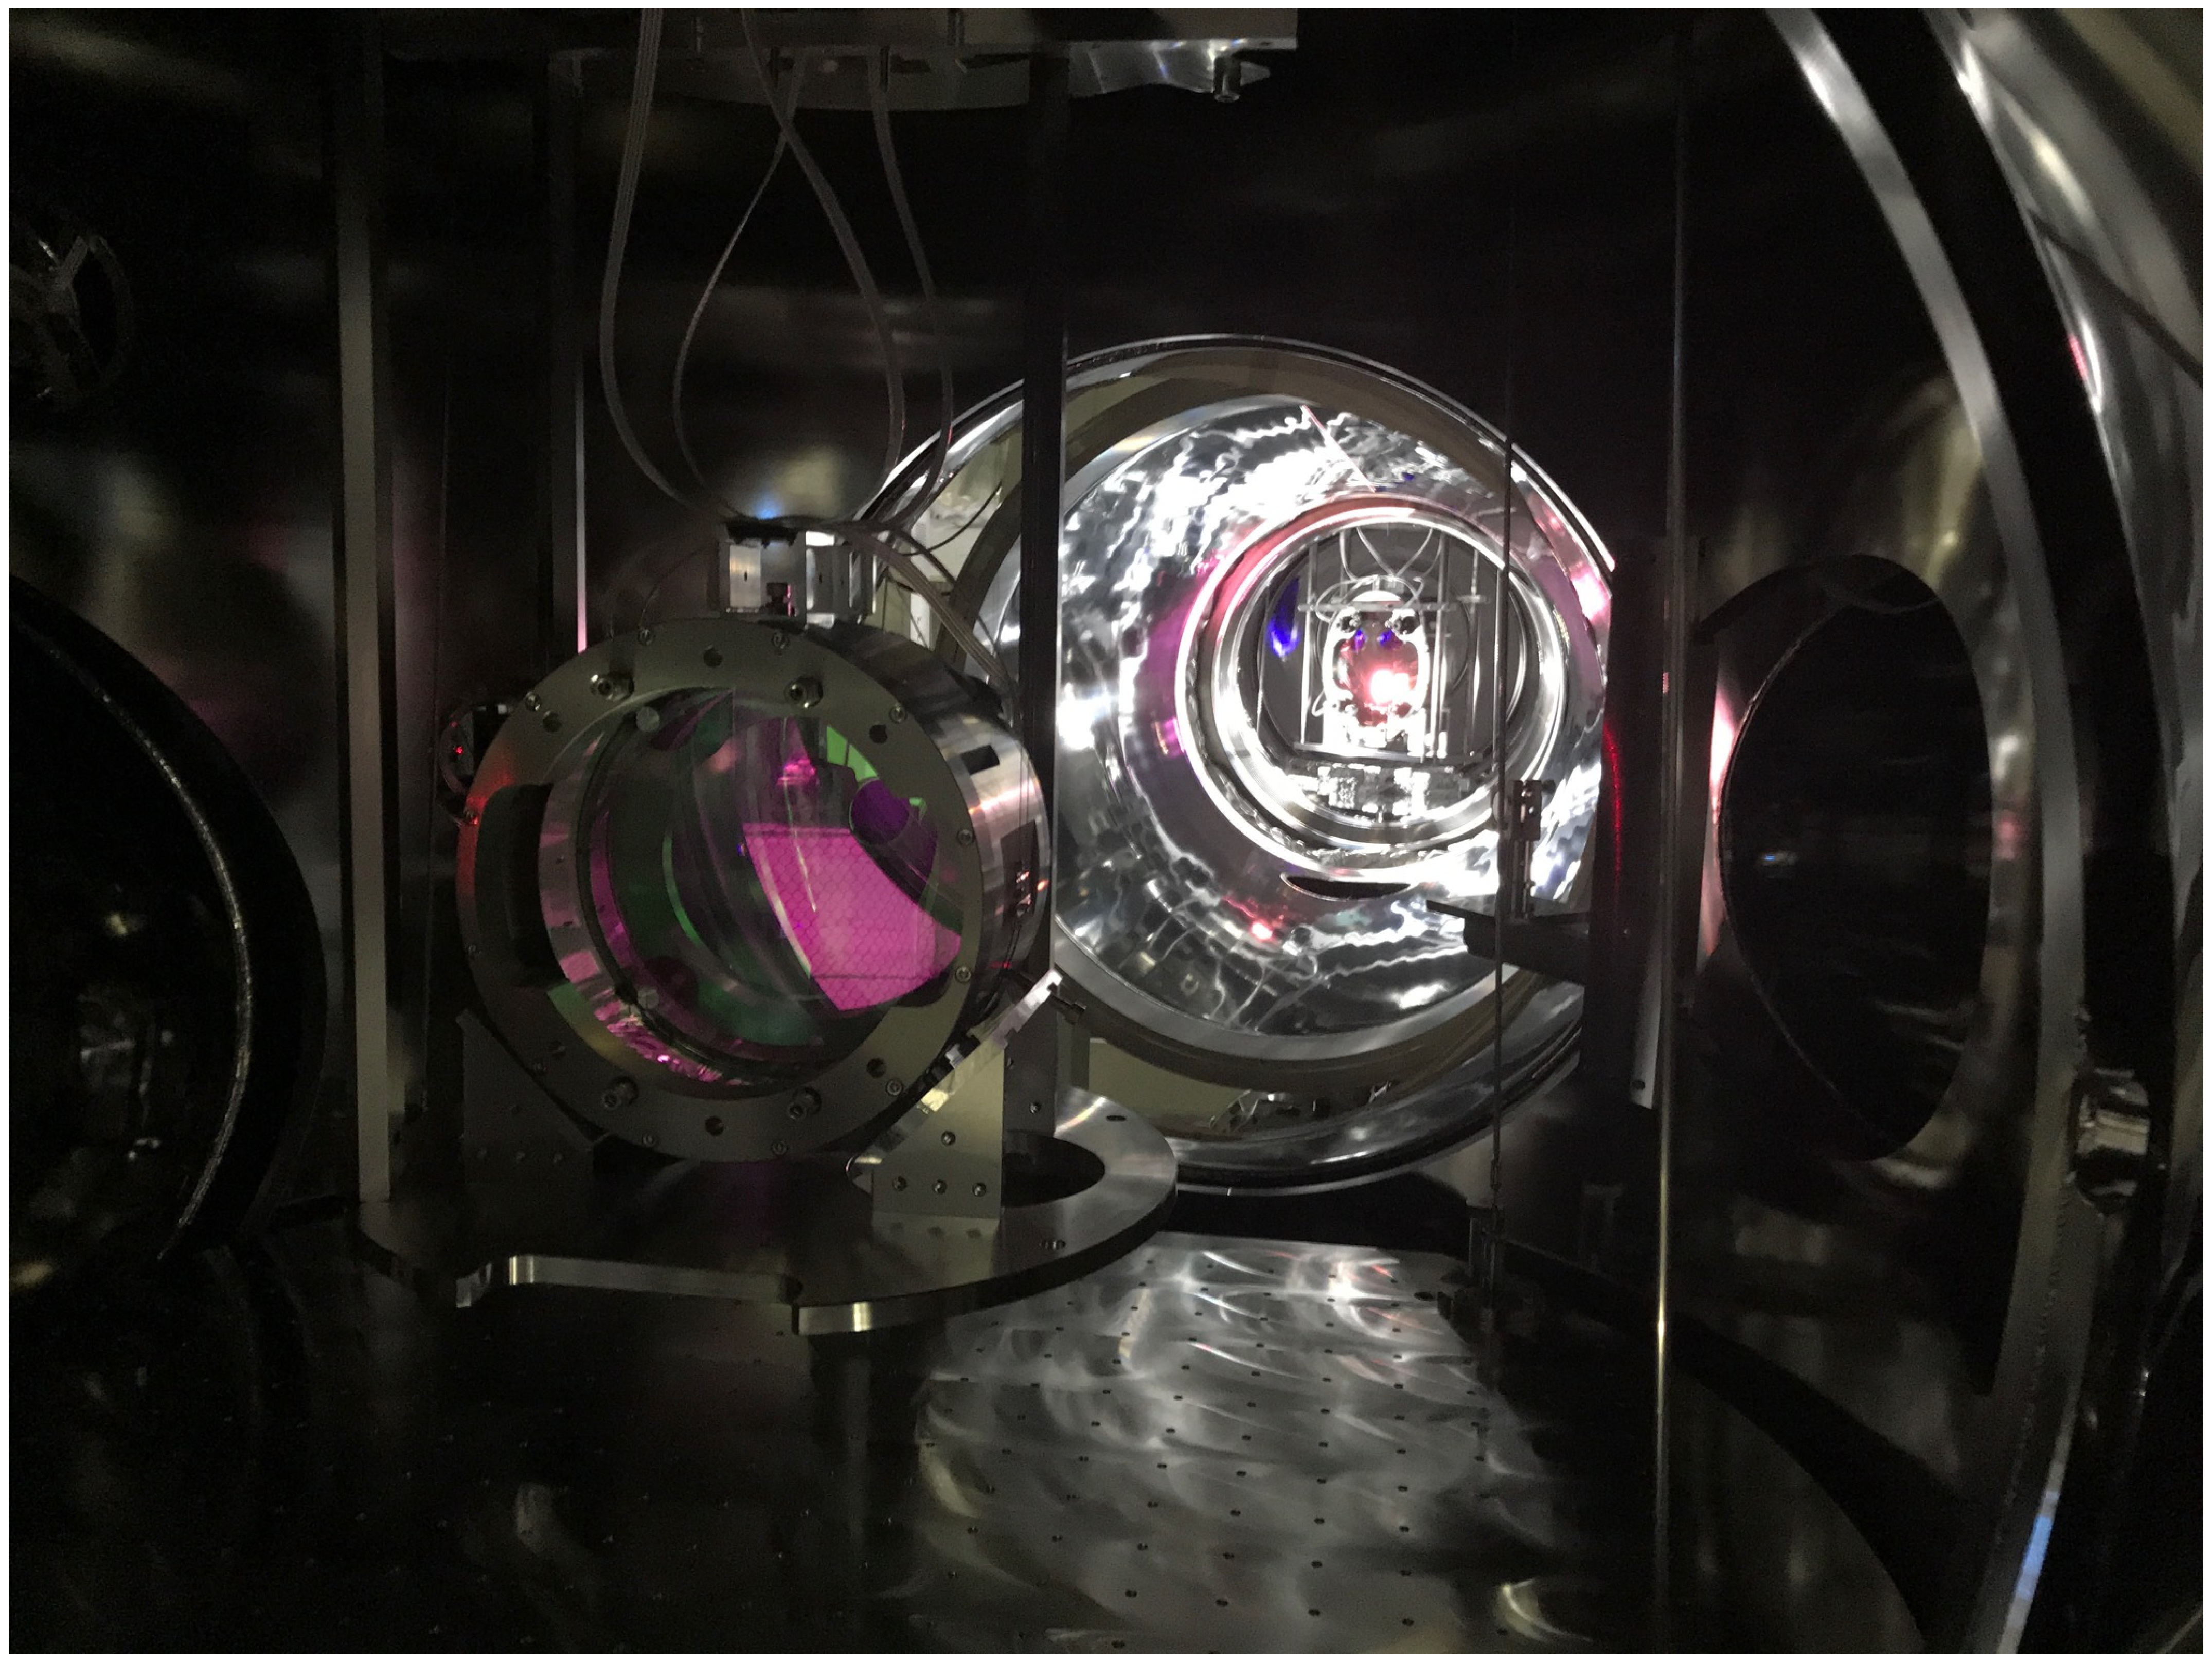
\includegraphics[width=8.5cm]{astrodiv/gw/overview/fig/pr2.eps}
%\caption{PR2 mirror suspended in a vacuum chamber. There is beam splitter behind the PR2 mirror.}
%\label{fig:bs}
%\end{center}
%\end{figure}
%
%    \begin{figure}
%\begin{center}
%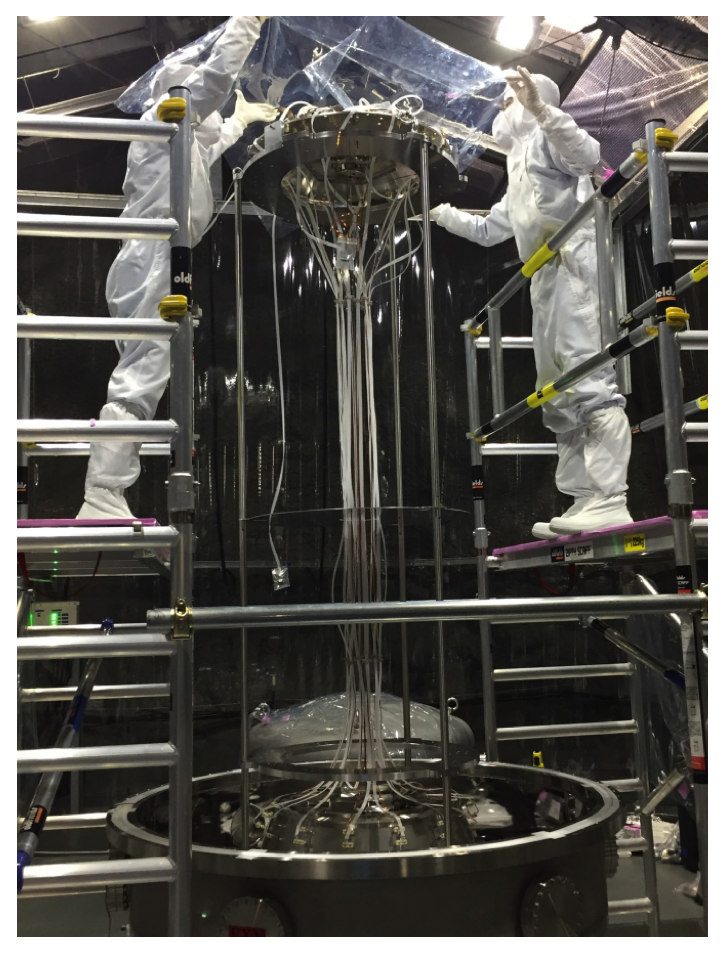
\includegraphics[width=8.5cm]{astrodiv/gw/overview/fig/typea.eps}
%\caption{A part of Type-A vibration isolation system.}
%\label{fig:bs}
%\end{center}
%\end{figure}



%In FY 2015 we installed many subsystems necessary for iKAGRA, including the connecting beam tubes, gate valves, input mode cleaner, input mode-matching telescope, power recycling folding mirrors, beam splitter, two end mirrors, suspension systems, other optics, optical levers, beam dumpers, analog electronics, digital control system, etc. Then we successfully locked the input mode cleaner, aligned the 3 km Michelson interferometer, and locked the interferometer.
%
%Then we performed a test run between Mar. 25 and Mar. 31, 2016. (The second test run was conducted in April 2016, but it will be reported in the annual report next year.) The input power to the beam splitter was 220 mW. The duty factor of the Michelson interferometer was 85.2 \%, and that of the input mode cleaner was 94.4 \%. The total lock time was 129.5 hours, and the longest lock was 3.6 hours. The typical strain sensitivity of the detector was $ 3\times 10^{-15} {\rm{Hz}}^{-1/2} $ at 100 Hz, which corresponds to a neutron star binary inspiral range of 0.77 pc.
%
%The interferometer was locked to the mid-fringe with a unity gain frequency of 8 Hz. All the suspended mirrors were controlled with the optical lever systems. The finesse and mode matching ratio of the pre-mode cleaner was 197 and 75 \%, respectively. The finesse and mode matching ratio of the input mode cleaner was 540 and 86.2 \%, respectively. The input mode cleaner mirrors, beam splitter, and end mirrors had Type-C suspension systems, while the power recycling folding mirror 3 had a Type-Bp' suspension system. The beam splitter, end mirrors, and power recycling folding mirror 3 were not in the vacuum because of insufficient commissioning time. The 80 Hz and 135 Hz monochromatic signals were applied to the control loop for the calibration of the interferometer. The interferometer lock was lost mainly because of the tidal drift of the mirrors. The noise spectrum was fluctuated by one order of magnitude. The sensitivity was limited mainly by intensity noise of laser light above 100 Hz.

%In the end of FY2015 we performed the first half of test run between Mar. 25 and Mar. 31, 2016. The details of the iKAGRA interferometer and the test run were described in the last annual report. In the beginning of FY 2016 we stopped the test run and improved the interferometer to reduce noise level and enhance stability. After the improvements, we performed the second half of test run from Apr. 11 to Apr. 25. Typical noise level at 100\,Hz was improved from $ 3\times 10^{-15} {\rm{Hz}}^{-1/2} $ to $ 7\times 10^{-16} {\rm{Hz}}^{-1/2} $ and an observation range of gravitational waves from binary coalescences of Neutron stars with 1.4 solar mass was extended from 0.77\,pc to 4.2\,pc. The duty cycle of the interferometer was increased from 85.2 \% to 90.4 \% even though Kumamoto earthquakes on Apr. 14 and 16 hit the test run. The longest lock of the interferometer reached 21.3 hours instead of 3.6 hours in the first half of the test run. 
%
%The scimon shift we took during the test run was the following. Each day was divided into three shift: 1:00 to 9:00, 9:00 to 17:00, and 17:00 to 1:00. In each shift slot one expert from ICRR, NAOJ, and KEK and two researchers from other universities/institutes were allocated. These scimons registered what happened as well as unusual events that they noticed during the shift. The scimon shift worked pretty smoothly. Finally, total of 65 people and cumulative total of 186 people from 35 institutes participated the shift works.
%
%All the data that was taken during the test run was stored and transferred to ICRR Kashiwa and Osaka City University in real time. The delayed mirroring of raw data was performed by Academia Sinica, Taiwan. KISTI, Korea was also copying the data. The transfer time from the KAGRA site to surface, ICRR Kashiwa, and Osaka City University was 0.3 sec, 2.5 sec, and 3 sec, respectively. The data management system worked very well.

%We started upgrading the interferometer from iKAGRA to bKAGRA after the test run, because we plan to operate the cryogenic 3\,km Michelson interferometer by the end of March 2018. The upgrading works are on going by many sub-groups. We give reports in the following sections from the vacuum sub-group, the input and output optics sub-group, the cryogenic sub-group, the digital control system sub-group, the detector characterization sub-group, and the mirror subgroup.


%The photos of  KAGRA taken in FY 2015 are shown (Fig.~\ref{fig:entrance} - Fig.~\ref{fig:PR3}).
%
%\begin{figure}
%\begin{center}
%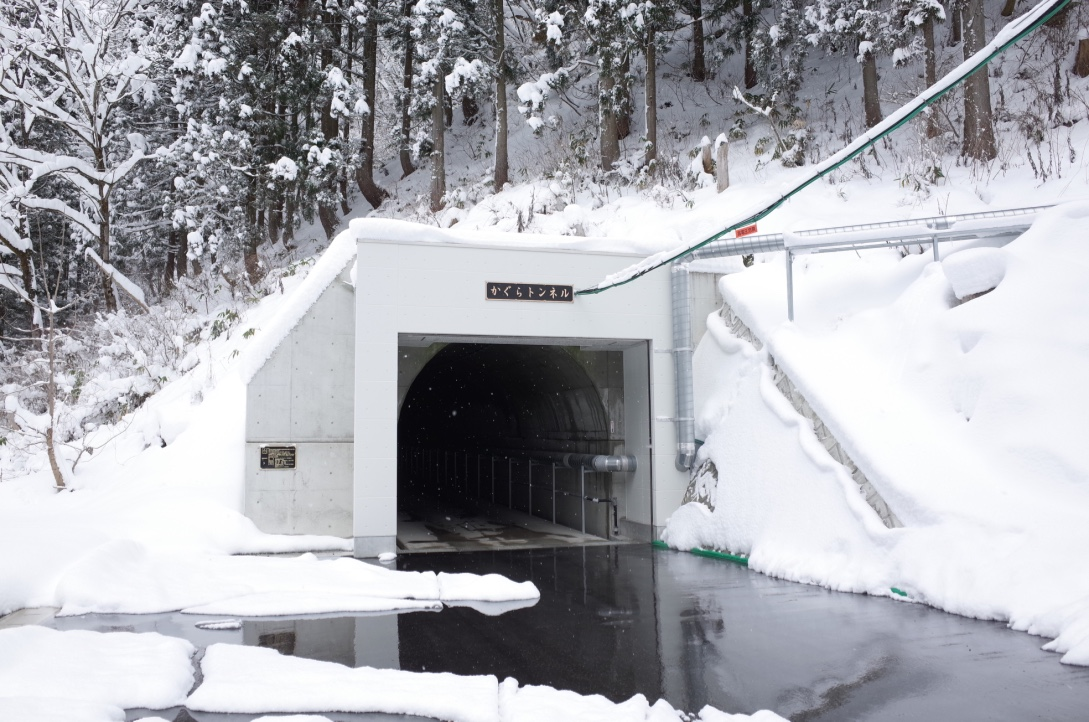
\includegraphics[width=8.5cm]{astrodiv/gw/Overview/fig/entrance.eps}
%\caption{Entrance of the KAGRA tunnel.}
%\label{fig:entrance}
%\end{center}
%\end{figure}
%
%\begin{figure}
%\begin{center}
%\includegraphics[width=8.5cm]{astrodiv/gw/Overview/fig/chambers.eps}
%\caption{Vacuum chambers in the central area.}
%\label{fig:chambers}
%\end{center}
%\end{figure}
%
%\begin{figure}
%\begin{center}
%\includegraphics[width=8.5cm]{astrodiv/gw/Overview/fig/cryostat.eps}
%\caption{Cryostat for the cryogenic mirror and the shaft for the vibration isolation system.}
%\label{fig:cryostat}
%\end{center}
%\end{figure}
%
%\begin{figure}
%\begin{center}
%\includegraphics[width=8.5cm]{astrodiv/gw/Overview/fig/slope.eps}
%\caption{Slope to the 2nd floor.}
%\label{fig:slope}
%\end{center}
%\end{figure}
%
%\begin{figure}
%\begin{center}
%\includegraphics[width=8.5cm]{astrodiv/gw/Overview/fig/beamtube.eps}
%\caption{3-km beam tube in the Y-arm tunnel.}
%\label{fig:beamtube}
%\end{center}
%\end{figure}
%
%\begin{figure}
%\begin{center}
%\includegraphics[width=8.5cm]{astrodiv/gw/Overview/fig/PSL.eps}
%\caption{Pre-stabilized laser for iKAGRA.}
%\label{fig:PSL}
%\end{center}
%\end{figure}
%
%\begin{figure}
%\begin{center}
%\includegraphics[width=8.5cm]{astrodiv/gw/Overview/fig/MC.eps}
%\caption{Mirrors and suspension systems of the input mode cleaner.}
%\label{fig:MC}
%\end{center}
%\end{figure}
%
%\begin{figure}
%\begin{center}
%\includegraphics[width=8.5cm]{astrodiv/gw/Overview/fig/PR3.eps}
%\caption{Power recycling folding mirror and its suspension system.}
%\label{fig:PR3}
%\end{center}
%\end{figure}

We also enhanced the international collaborations with the Einstein Telescope (ET) project, LIGO, Virgo, Korean and other Asian groups mainly based on the JSPS core-to-core program.

The rapidly progressing status of KAGAR were presented in many international conferences. Many papers about the progress of KAGRA were also published  \cite{quantum},  \cite{als}, \cite{damping}, \cite{cryo-op}, \cite{mzm}, \cite{contami}, \cite{sapphire mirror}, \cite{kagra status}. We also presented activities on our web-page.\cite{KAGRA}

\if 0
\begin{thebibliography}{99}


\bibitem{kagra_review} "KAGRA: 2.5 generation interferometric gravitational wave detector",
KAGRA collaboration, Nature Astronomy, Vol. 3, January 2019, 35-40

\bibitem{ikagra_paper} "Construction of KAGRA: an underground gravitational-wave observatory",
KAGRA collaboration,
Prog. Theor. Exp. Phys. 2018, 013F01 (2018)

\bibitem{phase1_paper} "First cryogenic test operation of underground km-scale gravitational-wave observatory KAGRA",
KAGRA collaboration, Class. Quantum Grav. 36 165008 (2019)


\bibitem{scenario_paper} "Prospects for observing and localizing gravitational-wave transients with Advanced LIGO, Advanced Virgo and KAGRA",
Abbott, B.P., Abbott, R., Abbott, T.D. et al. arXiv:1304.0670v10 [gr-qc]

\bibitem{o3_suspend} https://www.ligo.caltech.edu/news/ligo20200326

\bibitem{moa} https://gwdoc.icrr.u-tokyo.ac.jp/cgi-bin/DocDB/ShowDocument?docid=10663
\bibitem{moa_at} https://gwdoc.icrr.u-tokyo.ac.jp/cgi-bin/DocDB/ShowDocument?docid=10664
\bibitem{loi_o3} https://gwdoc.icrr.u-tokyo.ac.jp/cgi-bin/DocDB/ShowDocument?docid=10813

%2019
\bibitem{quantum} "Quantum noise reduction techniques in KAGRA", K Somiya, The European Physical Journal D volume 74, Article number: 10 (2020)
\bibitem{als} "An arm length stabilization system for KAGRA and future gravitational-wave detectors", T Akutsu et al., Class. Quantum Grav. 37 (2020) 035004 (19pp)

\bibitem{damping} "Vibration isolation system with a compact damping system for power recycling mirrors of KAGRA", Y Akiyama et al., Class. Quantum Grav. 36 (2019) 095015 (16pp)
\bibitem{cryo-op} "First cryogenic test operation of underground km-scale gravitational-wave observatory KAGRA", T Akutsu et al., Class. Quantum Grav. 36 (2019) 165008 (22pp)
\bibitem{mzm} "Design and experimental demonstration of a laser modulation system for future gravitational-wave detectors", K Yamamoto et al., Class. Quantum Grav. 36 (2019) 205009 (19pp)

\bibitem{contami} "Molecular adsorbed layer formation on cooled mirrors and its impacts on cryogenic gravitational wave telescopes", K Hasegawa et al., Phys. Rev. D 99, 022003
\bibitem{sapphire mirror} "Influence of nonuniformity in sapphire substrates for a gravitational wave telescope", K Somiya et al., Phys. Rev. D 100, 082005
%\bibitem{tilt} "Demonstration for a two-axis interferometric tilt sensor in KAGRA", Keiko Kokeyama,  Phys. Lett. A 382 (2018) 1950\UTF{2013}1955
%\bibitem{localizing} "Prospects for observing and localizing gravitational-wave transients with Advanced LIGO, Advanced Virgo and KAGRA", B. P. Abbott et al., Living Reviews in Relativity volume 21, Article number: 3 (2018) 

\bibitem{kagra status} "The status of KAGRA underground cryogenic gravitational wave telescope", T Akutsu et al., Journal of Physics: Conference Series, Volume 1342, XV International Conference on Topics in Astroparticle and Underground Physics 24-28 June 2017, Sudbury, ON, Canada
%2019



%
%
%
%\bibitem{xarm_com} "An arm length stabilization system for KAGRA and future gravitational-wave detectors",
%KAGRA collaboration,
%to be published in Class. Quantum Grav. (2019)



%
%\bibitem{michimura} "Mirror actuation design for the interferometer control of the KAGRA gravitational wave telescope",
%Yuta Michimura, Tomofumi Shimoda, Takahiro Miyamoto, Ayaka Shoda, Koki Okutomi, Yoshinori Fujii, Hiroki Tanaka, Mark A. Barton, Ryutaro Takahashi, Yoichi Aso, Tomotada Akutsu, Masaki Ando, Yutaro Enomoto, Raffaele Flaminio, Kazuhiro Hayama, Eiichi Hirose, Yuki Inoue, Takaaki Kajita, Masahiro Kamiizumi, Seiji Kawamura, Keiko Kokeyama, Kentaro Komori, Rahul Kumar, Osamu Miyakawa, Koji Nagano, Masayuki Nakano, Naoko Ohishi, Ching Pin Ooi, Fabian Erasmo Pena Arellano, Yoshio Saito, Katsuhiko Shimode, Kentaro Somiya, Hiroki Takeda, Takayuki Tomaru, Takashi Uchiyama, Takafumi Ushiba, Kazuhiro Yamamoto, Takaaki Yokozawa, Hirotaka Yuzurihara, Classical and Quantum Gravity 34, 225001(2017)
%
%\bibitem{gif} "Design and operation of a 1500-m laser strainmeter installed at underground site in Kamioka",
%Akito Araya, Akiteru Takamori, Wataru Morii, Kouseki Miyo, Masatake Ohashi, Kazuhiro Hayama, Takashi Uchiyama, Shinji Miyoki and Yoshio Saito, Earth, Planets and Space 69, 77 (2017)
%




\bibitem{KAGRA} http://gwcenter.icrr.u-tokyo.ac.jp/en/

\end{thebibliography}
\fi


%\cite{}


